\section*{Annexes} % Pas de numérotation
\phantomsection
\addcontentsline{toc}{section}{Annexes}
\appendix
\renewcommand\thefigure{\thesection.\arabic{figure}}
\renewcommand\thelstlisting{\thesection.\arabic{lstlisting}}
\setcounter{figure}{0}
\setcounter{lstlisting}{0}
\setcounter{section}{1}
%\setcounter{subsection}{1}

\subsection{\label{iot-lab}Distribution des nœuds FIT iot-lab}


\begin{figure}[ht!]
\centering
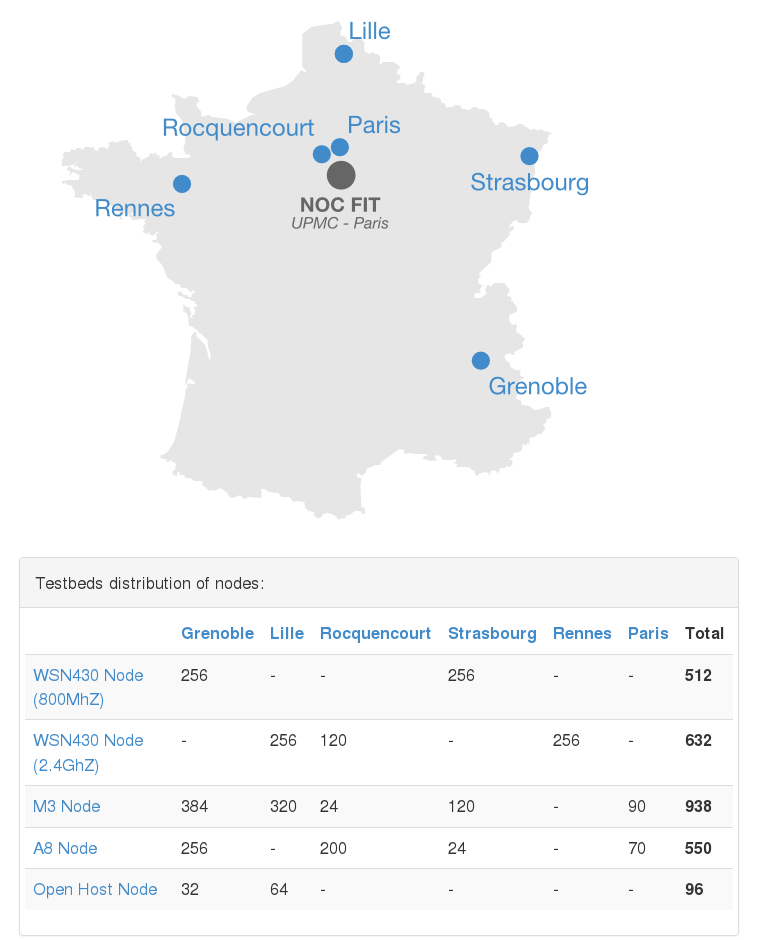
\includegraphics[scale=0.6]{images/iot-lab.png}
\caption{Source: https://www.iot-lab.info/deployment/}
\end{figure}

\subsection{\label{massif}Sortie de Massif}
\begin{figure}[ht!]
\centering
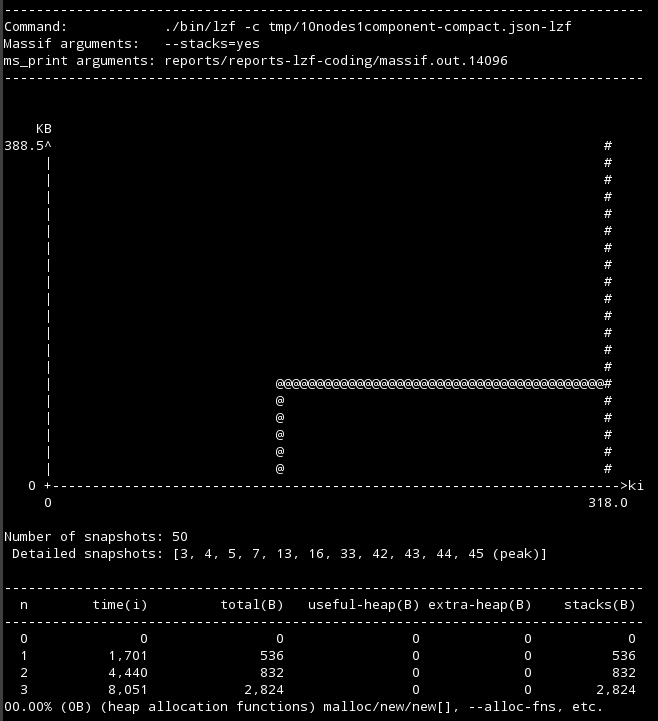
\includegraphics[scale=0.7]{images/msprint.png}
\caption{Exemple d'extrait de sortie de Massif, ici l'utilisation maximum de RAM est au snapshot 45 et est d'environ 400KB.}
\end{figure}

\begin{landscape}
\subsection{\label{comp-tabde}Compression de modèles}
\begin{figure}[ht!]
\centering
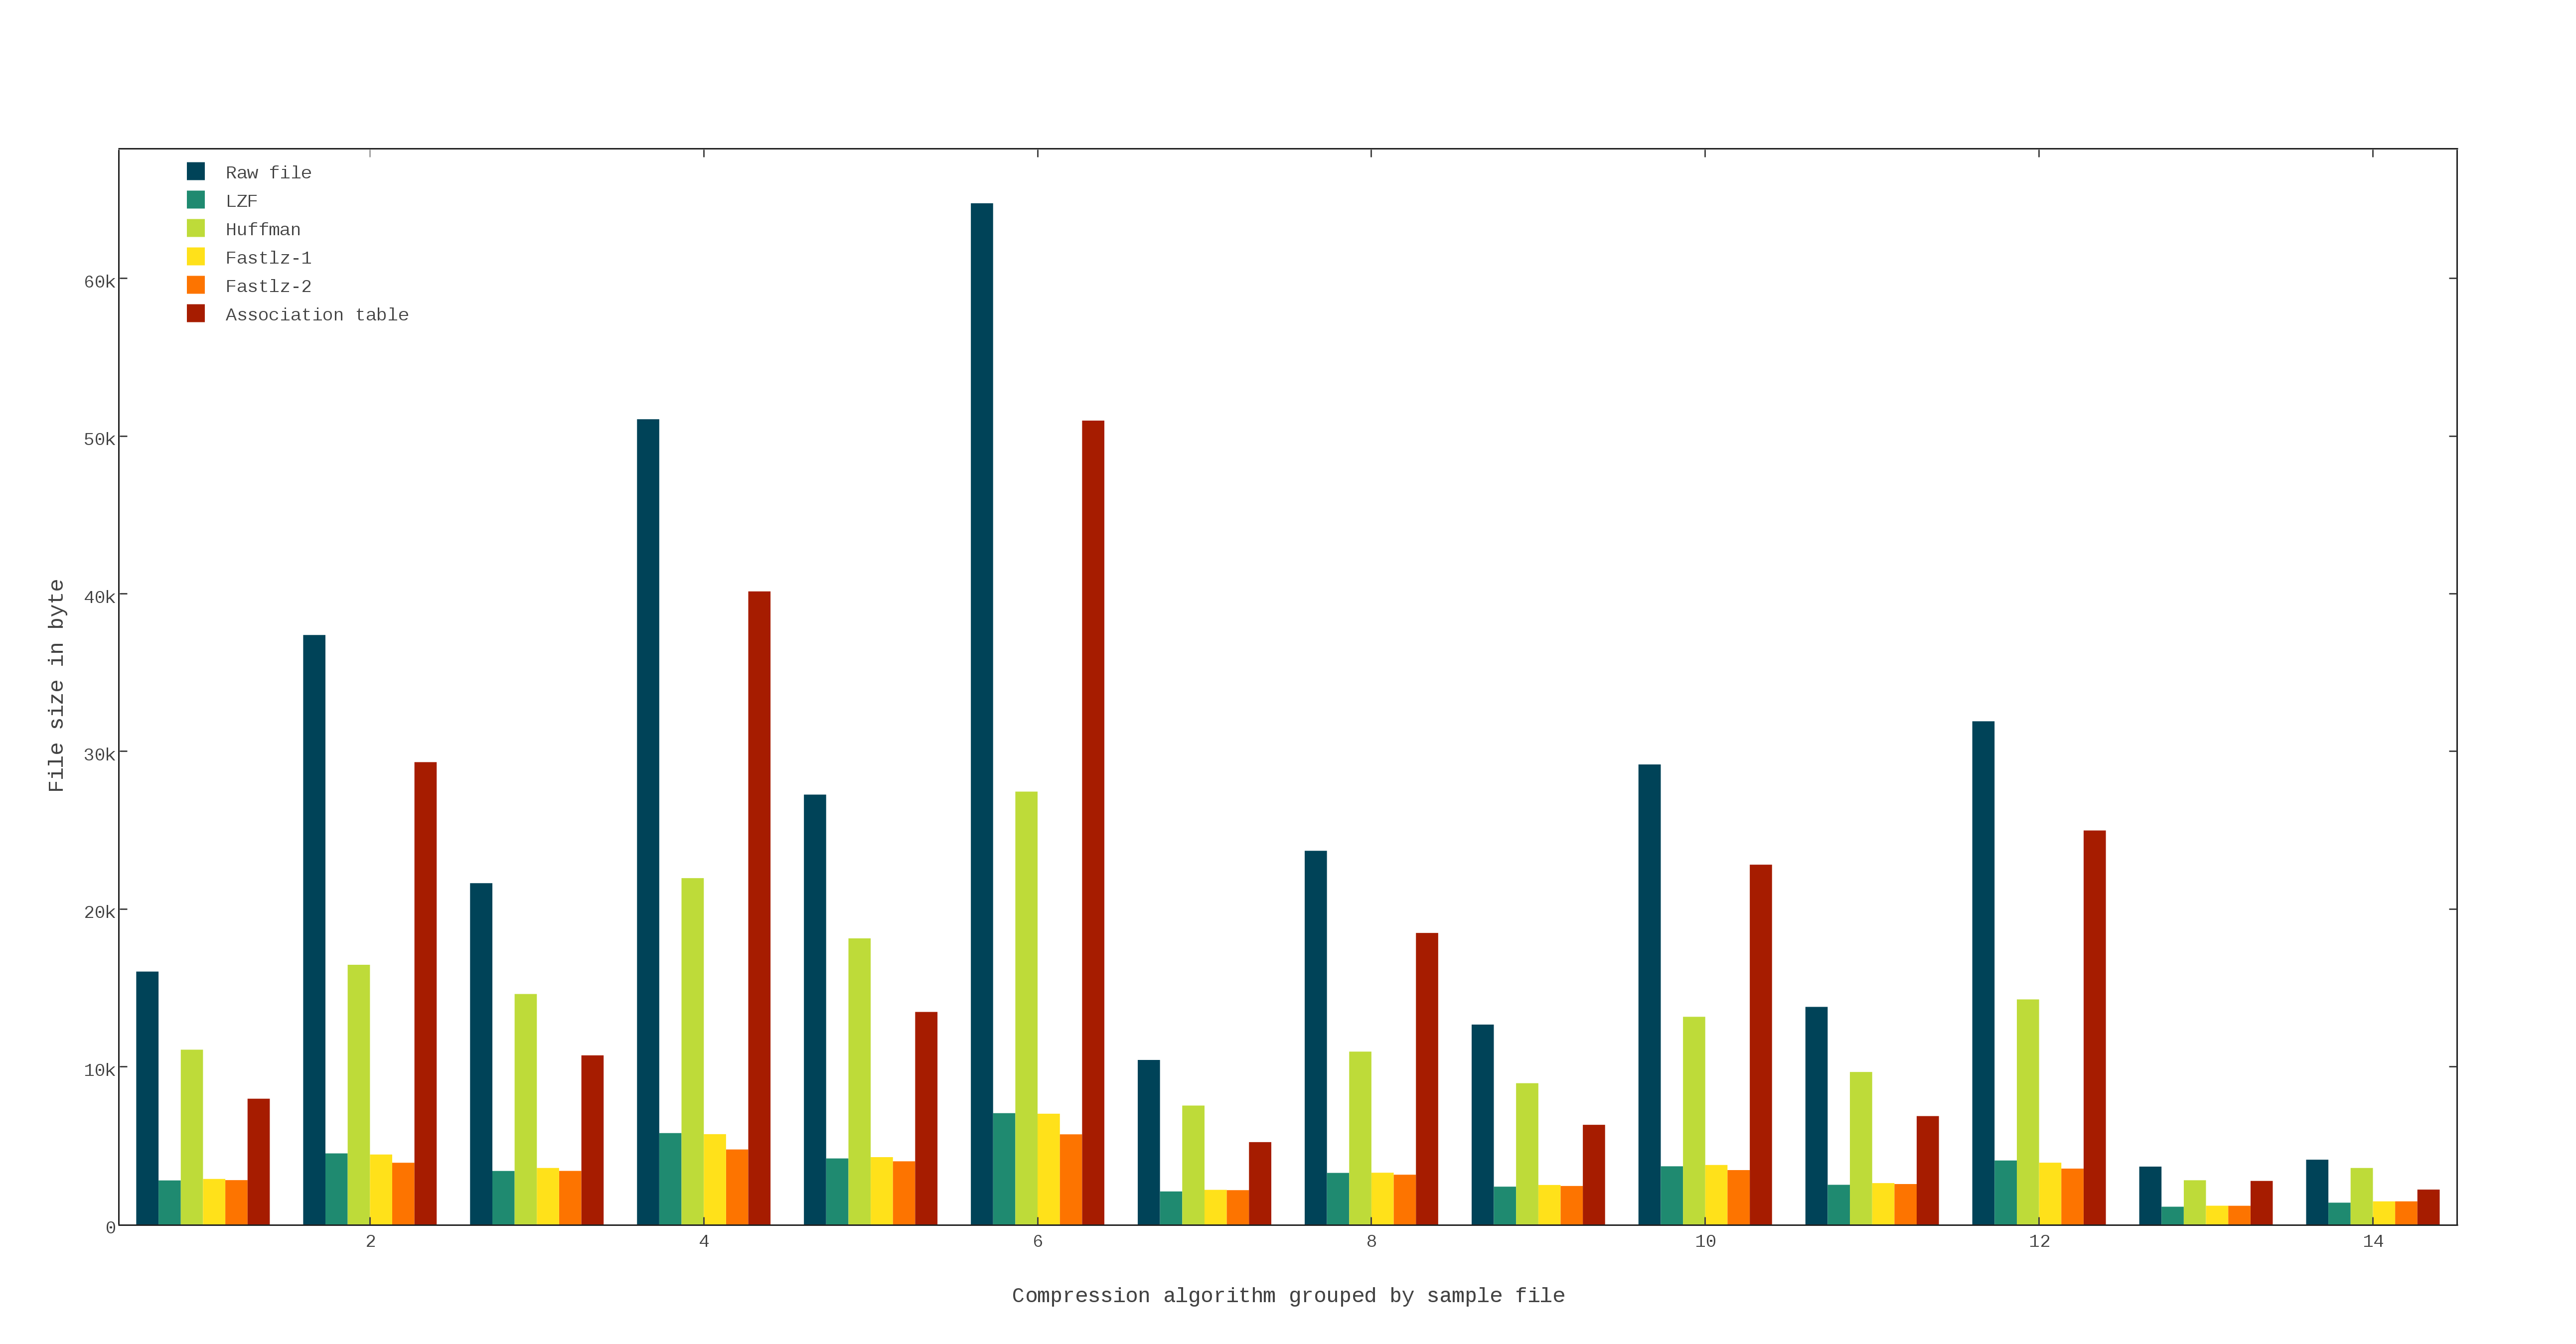
\includegraphics[scale=0.45]{images/compression.png}
\caption{Mesure de compression de modèles à l'aide de différents algorithmes}
\end{figure}
\end{landscape}

\begin{landscape}
\subsection{\label{kevoree-full-cd}Méta-modèle Kevoree}
\begin{figure}[ht!]
\centering
\fontsize{1mm}{4mm}\selectfont
\def\svgscale{0.28}
\input{images/kevoree-full-cd.pdf_tex}
\caption{Représentation du méta-modèle de Kevoree.}
\end{figure}
\end{landscape}

\lstset{
 language=C,
 captionpos=b,
 numbers=left,
 otherkeywords={},
 caption={Extrait du fichier Dictionary.h.}
}

\subsection{\label{dico-struct}Exemple de \texttt{struct} représentant une classe}
\begin{lstlisting}[frame=single]
typedef DictionaryValue* (*ftprDictionaryFindValuesByID)(Dictionary*, char*);
void initDictionary(Dictionary*);
Dictionary* new_Dictionary(void);

typedef struct _VT_Dictionary {
	VT_KMFContainer *super;
	/* KMFContainer */
	fptrKMFMetaClassName metaClassName;
	fptrKMFInternalGetKey internalGetKey;
	fptrKMFGetPath getPath;
	int (*fptrToJSON)(void*);
	fptrFindByPath findByPath;
	fptrDelete delete;
	/*Dictionary*/
	ftprDictionaryAddValues dictionaryAddValues;
	ftprDictionaryRemoveValues dictionaryRemoveValues;
	ftprDictionaryFindValuesByID dictionaryFindValuesByID;
} VT_Dictionary;

typedef struct _Dictionary {
	VT_Dictionary *VT;
	/* KMFContainer */
	KMFContainer *eContainer;
	/* Dictionary */
	char generated_KMF_ID[9];
	map_t values;
} Dictionary;
\end{lstlisting}